\section{Wearables}\label{sec:wearables}
If we take a look at the current state of wearables, 
or the most popular wearable devices right now, 
we can create an image of what we can actually monitor, track, 
control or in other ways do with devices that we can wear. 
One of the latest and most advanced wearable is the HIRIS \cite{hirisweb}. 
The HIRIS is a wearable computer able to track 3D movements in real-time, 
making it possible to perform 3D gestures to \eg perform commands. 
By using several HIRIS, you can create a full-body tracking system.
Aside from 3D tracking, HIRIS also tracks heart rate and temperature, 
and can connect to other devices and control these. 
Another advanced wearable tracker is the Jawbone UP3 \cite{JAWBONE}. 
This wearable is also able to track your heart rate, activity, sleep and temperature, 
but unlike the Hiris cannot control any other devices. 
One of most interesting smartwatches, due to developer options, is the Pebble Smartwatch \cite{PEBBLE}. 
This smartwatch works with iPhones and Android smartphones, 
and comes with a variety of applications for tracking fitness and control music among other things. 
Aside from this, the watch also comes with an accelerometer and a magnetometer, 
meaning that is can track your motions and directions. 

By analyzing the list of 348 different wearables from Vandrico \cite{LISTOFWEARABLES}\footnote{September 2015 numbers}, 
we can determine which sensors and components are most common among wearables, 
and where on the body they are worn. 
It is important to note that all of this information comes from Vandrico's database, 
and may differ from other findings. 
\Cref{fig:wearables-category} shows which categories these wearables fit in. 
The most common one, lifestyle, describes wearables such as smartwatches, 
or other devices that are meant to be used and worn on a daily basis. 
Some devices may fit more than one category.

\begin{figure}[!htb]
    \centering
    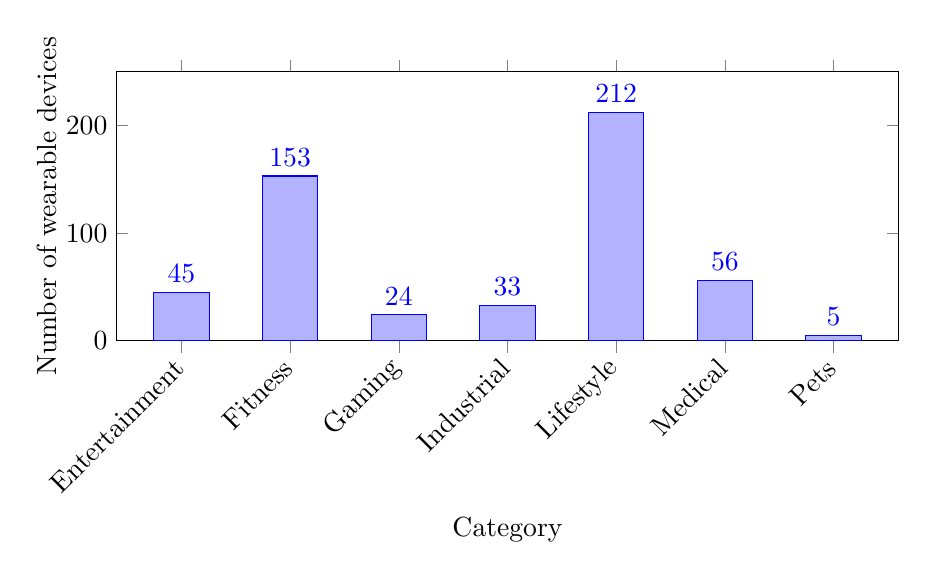
\begin{tikzpicture}
    \begin{axis}[
        height=5cm,
        width=0.95\textwidth,
        xlabel={Category},
        xticklabel style={rotate=45, anchor=east, yshift=-0.5ex},
        ylabel={Number of wearable devices},
        yticklabel style={align=right,inner sep=0pt,xshift=-0.3em},
        nodes near coords align={vertical},
        nodes near coords,
        xtick=data,
        symbolic x coords={Entertainment,Fitness,Gaming,Industrial,Lifestyle,Medical,Pets},
        ybar,
        ymax=250,
        ymin=0,
        bar width=20pt,
        ]
        \addplot coordinates {(Entertainment,45) (Fitness,153) (Gaming,24) (Industrial,33) (Lifestyle,212) (Medical,56) (Pets,5)};
    \end{axis}
\end{tikzpicture}
    \caption{Number of devices in each category. Data from \protect\cite{LISTOFWEARABLES}.}
    \label{fig:wearables-category}
\end{figure}

We have visualized the most common sensors and components in \Cref{fig:wearables-sensors}.
Due to its high usability, the accelerometer is a very important sensor, 
which is found in approximately half the wearables. 
The remaining sensors in \Cref{fig:wearables-sensors} are, unsurprisingly, sensors that we also find in smartphones, 
as they give a lot of options when it comes to developing applications. 

\begin{figure}[!htb]
    \centering
    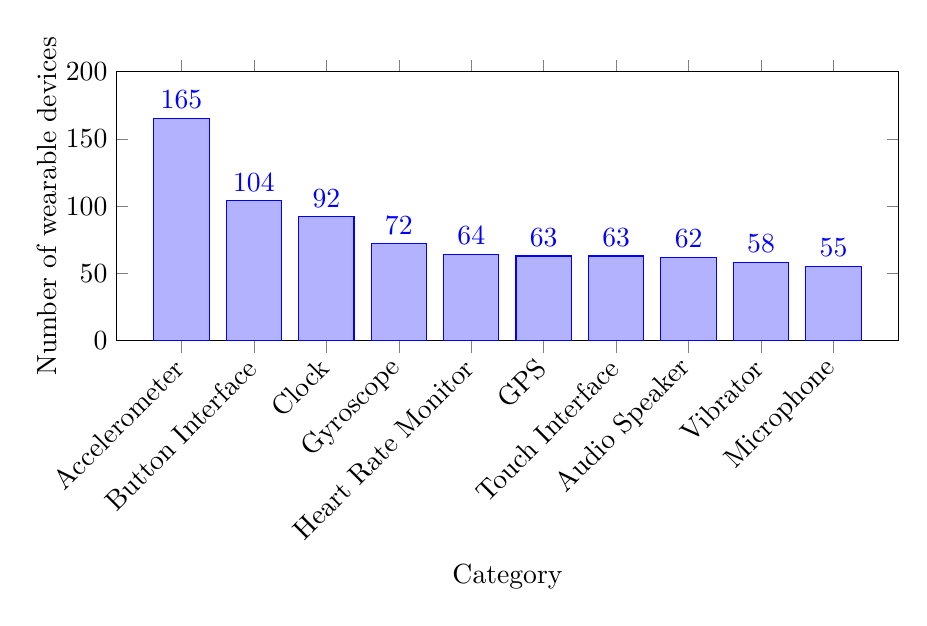
\begin{tikzpicture}
    \begin{axis}[
        height=5cm,
        width=0.95\textwidth,
        xlabel={Category},
        xticklabel style={rotate=45, anchor=east, yshift=-0.5ex},
        ylabel={Number of wearable devices},
        yticklabel style={align=right,inner sep=0pt,xshift=-0.3em},
        nodes near coords align={vertical},
        nodes near coords,
        xtick=data,
        symbolic x coords={Accelerometer,Button Interface,Clock,Gyroscope,Heart Rate Monitor,GPS,Touch Interface,Audio Speaker,Vibrator,Microphone},
        ybar,
        ymax=200,
        ymin=0,
        bar width=20pt,
        ]
        \addplot coordinates {(Accelerometer,165) (Button Interface,104) (Clock,92) (Gyroscope,72) (Heart Rate Monitor,64) (GPS,63) (Touch Interface,63) (Audio Speaker,62) (Vibrator,58) (Microphone,55)};
    \end{axis}
\end{tikzpicture}
    \caption{Top 10 mostly used sensors and components. Data from \protect\cite{LISTOFWEARABLES}.}
    \label{fig:wearables-sensors}
\end{figure}

\subsection{The Future of Wearables}
We have already mentioned that wearables is trending. 
From a report from Business Insider UK \cite{WEARABLESTREND}, 
Statista \cite{WEARABLESTRENDNUMBERS} has illustrated this trend as a bar plot, 
reproduced here as \Cref{fig:wearables-trend}.

\begin{figure}[!htb]
  \centering
  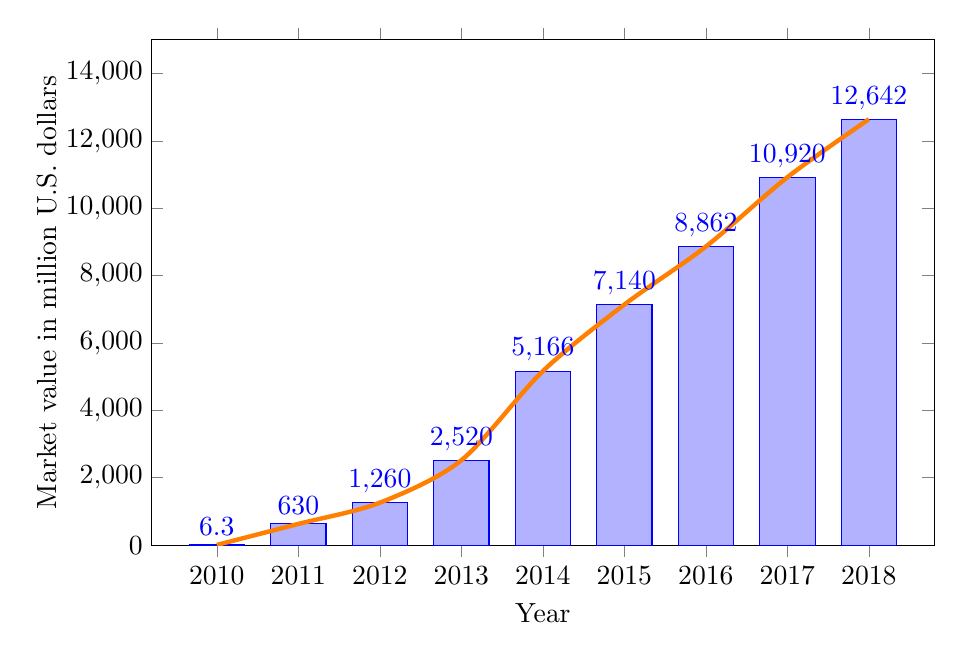
\begin{tikzpicture}
    \begin{axis}[
        height=8cm,
        width=0.95\textwidth,
        xlabel={Year},
        ylabel={Market value in million U.S. dollars},
        yticklabel style={align=right,inner sep=0pt,xshift=-0.3em},
        scaled y ticks = false,
        nodes near coords align={vertical},
        nodes near coords,
        xtick=data,
        symbolic x coords={2010, 2011, 2012, 2013, 2014, 2015, 2016, 2017, 2018},
%        ybar,
        ymax=15000,
        ymin=0,
%        bar width=20pt,
ybar, bar width=20pt
        ]
        \addplot coordinates {(2010, 6.3) (2011, 630) (2012, 1260) (2013, 2520) (2014, 5166) (2015, 7140) (2016, 8862) (2017, 10920) (2018, 12642)};
        \addplot [ultra thick,orange,line join=round,smooth, nodes near coords = ] coordinates {(2010, 6.3) (2011, 630) (2012, 1260) (2013, 2520) (2014, 5166) (2015, 7140) (2016, 8862) (2017, 10920) (2018, 12642)};
%        
    \end{axis}
\end{tikzpicture}
  \caption{Wearables trend based on sales and statistics. Data from \protect\cite{WEARABLESTRENDNUMBERS}.}
  \label{fig:wearables-trend}
\end{figure}

The figure shows the market value of wearables in the past years, 
but also utilizes statistics to determine the market value in the coming years. 
Based on this graph (and report), 
we see a very clear rise in the market value. 
This could lead to wearables becoming much more common,
attracting investors and developers, 
giving wearables a bright future. 

A report from PSFK \cite{PSFK} forecasts that by 2016, 
clothing wearables will become more advanced and more widely used. 
A few examples from the report include: 
``hug-jacket'' letting parents send ``hugs'' to their children via a mobile device, 
GPS tracking built into clothes of football players on the field for statistics, 
and a sweater that monitors the mood of the user and displays them, somewhat reminiscent of mood rings.

The report from PSFK also forecasts that by 2018, 
wearables will start to be embedded, \ie inserted into or attached to the human body. 
Examples of these types or wearables from the report are: 
prosthetic limbs, implanted headphones allowing users to echolocate, 
and a contact lens that lets the user zoom.

This section gave a short overview of the current and future state of wearables, 
what they are and which sensors are widely available. 

%%% Local Variables:
%%% mode: latex
%%% TeX-master: "../../master"
%%% End:
